\documentclass{standalone}
\usepackage{tikz}
\usepackage{ctex,siunitx}
\usepackage{tkz-euclide}
\usepackage{amsmath}
\usetikzlibrary{patterns, calc}
\usetikzlibrary {decorations.pathmorphing, decorations.pathreplacing, decorations.shapes,}
\begin{document}
\small
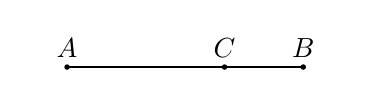
\begin{tikzpicture}[>=latex]
\useasboundingbox(-0.5,-0.2)rectangle(3.5,0.5);
\draw(0,0)--(3,0);
\fill(0,0)circle(1pt)node[above]{$A$};
\fill(2,0)circle(1pt)node[above]{$C$};
\fill(3,0)circle(1pt)node[above]{$B$};
\end{tikzpicture}
\end{document}